\documentclass[aspectratio=169, xcolor=dvipsnames]{beamer}

% --- Theme Setup ---
\usetheme{Madrid}
\usecolortheme{default}

% --- Packages ---
\usepackage{listings}
\usepackage{xcolor}
\usepackage{tikz}
\usetikzlibrary{shapes, arrows, positioning, fit}
\usepackage{booktabs}

% --- Code Highlighting Style ---
\definecolor{codegreen}{rgb}{0,0.6,0}
\definecolor{codegray}{rgb}{0.5,0.5,0.5}
\definecolor{codepurple}{rgb}{0.58,0,0.82}
\definecolor{backcolour}{rgb}{0.95,0.95,0.92}

\lstdefinestyle{mystyle}{
    backgroundcolor=\color{backcolour},   
    commentstyle=\color{codegreen},
    keywordstyle=\color{magenta},
    numberstyle=\tiny\color{codegray},
    stringstyle=\color{codepurple},
    basicstyle=\ttfamily\footnotesize,
    breakatwhitespace=false,         
    breaklines=true,                 
    captionpos=b,                    
    keepspaces=true,                 
    numbers=left,                    
    numbersep=5pt,                  
    showspaces=false,                
    showstringspaces=false,
    showtabs=false,                  
    tabsize=2,
    escapechar=|
}
\lstset{style=mystyle}

% --- Notes Setup ---
% Enable this to see notes in PDF if debug is needed, otherwise hide for video generation source
\setbeameroption{hide notes} 

\title{Beamer Feature Showcase}
\subtitle{Reference for LLM-Generated Video Slides}
\author{System Reference}
\date{\today}

\begin{document}

% ==========================================
% SLIDE 1: Title & Protocol
% ==========================================
\begin{frame}
    \titlepage
    \begin{center}
        \small This presentation demonstrates features for automated video generation.
    \end{center}
    
    \note{
        [click] Narrator: Welcome to the Beamer Feature Showcase. This document serves as a reference for creating video-ready slides.
        [click] Narrator: We will demonstrate the standard protocol for speaker notes, incremental reveals, and dynamic code visualization.
    }
\end{frame}

% ==========================================
% SLIDE 2: Incremental Content
% ==========================================
\begin{frame}{Incremental Reveals}
    To keep the video engaging, reveal content step-by-step using \texttt{<+->}.
    
    \begin{itemize}
        \item<1-> \textbf{Step 1}: Introduce the concept.
        \item<2-> \textbf{Step 2}: Expand on details.
        \item<3-> \textbf{Step 3}: Conclude the point.
    \end{itemize}
    
    \vspace{1em}
    \onslide<4->{
        \begin{alertblock}{Key Takeaway}
            Incremental reveals prevent cognitive overload and sync with the narration.
        \end{alertblock}
    }

    \note{
        Narrator: Let's talk about incremental reveals.
        [click] Narrator: First, we introduce the concept.
        [click] Narrator: Then, we expand on the details as the audience processes the information.
        [click] Narrator: Finally, we conclude the point.
        [click] Narrator: The key takeaway is that this technique keeps the video moving and prevents the viewer from reading ahead.
    }
\end{frame}

% ==========================================
% SLIDE 3: Code Evolution (Magic Move Sim)
% ==========================================
\begin{frame}[fragile]{Code Evolution}
    We can simulate "Magic Move" by showing code changes across overlays.
    
    \begin{onlyenv}<1>
        \begin{lstlisting}[language=Python, title={Initial State}]
def calculate_area(radius):
    pi = 3.14
    return pi * radius * radius
        \end{lstlisting}
    \end{onlyenv}
    
    \begin{onlyenv}<2>
        \begin{lstlisting}[language=Python, title={Refactored (Import Math)}]
import math

def calculate_area(radius):
    return math.pi * radius * radius
        \end{lstlisting}
    \end{onlyenv}
    
    \begin{onlyenv}<3>
        \begin{lstlisting}[language=Python, title={Type Hinting Added}]
import math

def calculate_area(radius: float) -> float:
    return math.pi * radius ** 2
        \end{lstlisting}
    \end{onlyenv}

    \note{
        Narrator: Code examples should evolve. Here is our initial implementation.
        [click] Narrator: We refactor it to use the math library for better precision.
        [click] Narrator: Finally, we add type hinting and optimize the exponentiation.
    }
\end{frame}

% ==========================================
% SLIDE 4: Visual Annotations (TikZ)
% ==========================================
\begin{frame}{Visual Annotations}
    Use TikZ to draw attention to specific elements.
    
    \vspace{1em}
    \centering
    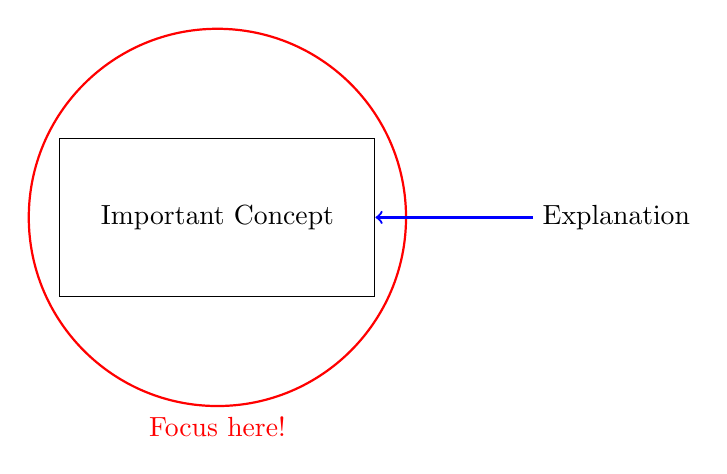
\begin{tikzpicture}
        \node[draw, rectangle, minimum width=4cm, minimum height=2cm] (box) {Important Concept};
        
        \node<2>[draw, circle, red, thick, fit=(box), label=below:\textcolor{red}{Focus here!}] {};
        
        \node<3>[right=of box, xshift=1cm] (note) {Explanation};
        \draw<3>[->, thick, blue] (note) -- (box);
    \end{tikzpicture}

    \note{
        Narrator: Sometimes text isn't enough.
        [click] Narrator: We can draw a circle around the core concept to direct the eye.
        [click] Narrator: Or use arrows to connect related ideas dynamically.
    }
\end{frame}

% ==========================================
% SLIDE 5: Layouts
% ==========================================
\begin{frame}[fragile]{Comparing Approaches}
    Use columns to compare side-by-side.
    
    \begin{columns}
        \begin{column}{0.48\textwidth}
            \textbf{Approach A (Recursive)}
            \begin{lstlisting}[language=Python, basicstyle=\tiny\ttfamily]
def fib(n):
    if n <= 1: return n
    return fib(n-1) + fib(n-2)
            \end{lstlisting}
        \end{column}
        
        \begin{column}{0.48\textwidth}
            \textbf{Approach B (Iterative)}
            \begin{lstlisting}[language=Python, basicstyle=\tiny\ttfamily]
def fib(n):
    a, b = 0, 1
    for _ in range(n):
        a, b = b, a + b
    return a
            \end{lstlisting}
        \end{column}
    \end{columns}
    
    \vspace{1em}
    \onslide<2->{
        \centering
        \textbf{Verdict:} Approach B is much faster.
    }

    \note{
        Narrator: Side-by-side comparisons are essential. On the left, we have a recursive approach.
        Narrator: On the right, an iterative one.
        [click] Narrator: As we can see, the iterative approach is superior for performance.
    }
\end{frame}

\end{document}
